\documentclass[]{article}
\usepackage{lmodern}
\usepackage{amssymb,amsmath}
\usepackage{ifxetex,ifluatex}
\usepackage{fixltx2e} % provides \textsubscript
\ifnum 0\ifxetex 1\fi\ifluatex 1\fi=0 % if pdftex
  \usepackage[T1]{fontenc}
  \usepackage[utf8]{inputenc}
\else % if luatex or xelatex
  \ifxetex
    \usepackage{mathspec}
  \else
    \usepackage{fontspec}
  \fi
  \defaultfontfeatures{Ligatures=TeX,Scale=MatchLowercase}
\fi
% use upquote if available, for straight quotes in verbatim environments
\IfFileExists{upquote.sty}{\usepackage{upquote}}{}
% use microtype if available
\IfFileExists{microtype.sty}{%
\usepackage{microtype}
\UseMicrotypeSet[protrusion]{basicmath} % disable protrusion for tt fonts
}{}
\usepackage[margin=1in]{geometry}
\usepackage{hyperref}
\hypersetup{unicode=true,
            pdftitle={Stat 343: MLE for Simple Linear Regression},
            pdfborder={0 0 0},
            breaklinks=true}
\urlstyle{same}  % don't use monospace font for urls
\usepackage{color}
\usepackage{fancyvrb}
\newcommand{\VerbBar}{|}
\newcommand{\VERB}{\Verb[commandchars=\\\{\}]}
\DefineVerbatimEnvironment{Highlighting}{Verbatim}{commandchars=\\\{\}}
% Add ',fontsize=\small' for more characters per line
\usepackage{framed}
\definecolor{shadecolor}{RGB}{248,248,248}
\newenvironment{Shaded}{\begin{snugshade}}{\end{snugshade}}
\newcommand{\KeywordTok}[1]{\textcolor[rgb]{0.13,0.29,0.53}{\textbf{#1}}}
\newcommand{\DataTypeTok}[1]{\textcolor[rgb]{0.13,0.29,0.53}{#1}}
\newcommand{\DecValTok}[1]{\textcolor[rgb]{0.00,0.00,0.81}{#1}}
\newcommand{\BaseNTok}[1]{\textcolor[rgb]{0.00,0.00,0.81}{#1}}
\newcommand{\FloatTok}[1]{\textcolor[rgb]{0.00,0.00,0.81}{#1}}
\newcommand{\ConstantTok}[1]{\textcolor[rgb]{0.00,0.00,0.00}{#1}}
\newcommand{\CharTok}[1]{\textcolor[rgb]{0.31,0.60,0.02}{#1}}
\newcommand{\SpecialCharTok}[1]{\textcolor[rgb]{0.00,0.00,0.00}{#1}}
\newcommand{\StringTok}[1]{\textcolor[rgb]{0.31,0.60,0.02}{#1}}
\newcommand{\VerbatimStringTok}[1]{\textcolor[rgb]{0.31,0.60,0.02}{#1}}
\newcommand{\SpecialStringTok}[1]{\textcolor[rgb]{0.31,0.60,0.02}{#1}}
\newcommand{\ImportTok}[1]{#1}
\newcommand{\CommentTok}[1]{\textcolor[rgb]{0.56,0.35,0.01}{\textit{#1}}}
\newcommand{\DocumentationTok}[1]{\textcolor[rgb]{0.56,0.35,0.01}{\textbf{\textit{#1}}}}
\newcommand{\AnnotationTok}[1]{\textcolor[rgb]{0.56,0.35,0.01}{\textbf{\textit{#1}}}}
\newcommand{\CommentVarTok}[1]{\textcolor[rgb]{0.56,0.35,0.01}{\textbf{\textit{#1}}}}
\newcommand{\OtherTok}[1]{\textcolor[rgb]{0.56,0.35,0.01}{#1}}
\newcommand{\FunctionTok}[1]{\textcolor[rgb]{0.00,0.00,0.00}{#1}}
\newcommand{\VariableTok}[1]{\textcolor[rgb]{0.00,0.00,0.00}{#1}}
\newcommand{\ControlFlowTok}[1]{\textcolor[rgb]{0.13,0.29,0.53}{\textbf{#1}}}
\newcommand{\OperatorTok}[1]{\textcolor[rgb]{0.81,0.36,0.00}{\textbf{#1}}}
\newcommand{\BuiltInTok}[1]{#1}
\newcommand{\ExtensionTok}[1]{#1}
\newcommand{\PreprocessorTok}[1]{\textcolor[rgb]{0.56,0.35,0.01}{\textit{#1}}}
\newcommand{\AttributeTok}[1]{\textcolor[rgb]{0.77,0.63,0.00}{#1}}
\newcommand{\RegionMarkerTok}[1]{#1}
\newcommand{\InformationTok}[1]{\textcolor[rgb]{0.56,0.35,0.01}{\textbf{\textit{#1}}}}
\newcommand{\WarningTok}[1]{\textcolor[rgb]{0.56,0.35,0.01}{\textbf{\textit{#1}}}}
\newcommand{\AlertTok}[1]{\textcolor[rgb]{0.94,0.16,0.16}{#1}}
\newcommand{\ErrorTok}[1]{\textcolor[rgb]{0.64,0.00,0.00}{\textbf{#1}}}
\newcommand{\NormalTok}[1]{#1}
\usepackage{graphicx,grffile}
\makeatletter
\def\maxwidth{\ifdim\Gin@nat@width>\linewidth\linewidth\else\Gin@nat@width\fi}
\def\maxheight{\ifdim\Gin@nat@height>\textheight\textheight\else\Gin@nat@height\fi}
\makeatother
% Scale images if necessary, so that they will not overflow the page
% margins by default, and it is still possible to overwrite the defaults
% using explicit options in \includegraphics[width, height, ...]{}
\setkeys{Gin}{width=\maxwidth,height=\maxheight,keepaspectratio}
\IfFileExists{parskip.sty}{%
\usepackage{parskip}
}{% else
\setlength{\parindent}{0pt}
\setlength{\parskip}{6pt plus 2pt minus 1pt}
}
\setlength{\emergencystretch}{3em}  % prevent overfull lines
\providecommand{\tightlist}{%
  \setlength{\itemsep}{0pt}\setlength{\parskip}{0pt}}
\setcounter{secnumdepth}{0}
% Redefines (sub)paragraphs to behave more like sections
\ifx\paragraph\undefined\else
\let\oldparagraph\paragraph
\renewcommand{\paragraph}[1]{\oldparagraph{#1}\mbox{}}
\fi
\ifx\subparagraph\undefined\else
\let\oldsubparagraph\subparagraph
\renewcommand{\subparagraph}[1]{\oldsubparagraph{#1}\mbox{}}
\fi

%%% Use protect on footnotes to avoid problems with footnotes in titles
\let\rmarkdownfootnote\footnote%
\def\footnote{\protect\rmarkdownfootnote}

%%% Change title format to be more compact
\usepackage{titling}

% Create subtitle command for use in maketitle
\newcommand{\subtitle}[1]{
  \posttitle{
    \begin{center}\large#1\end{center}
    }
}

\setlength{\droptitle}{-2em}

  \title{Stat 343: MLE for Simple Linear Regression}
    \pretitle{\vspace{\droptitle}\centering\huge}
  \posttitle{\par}
    \author{}
    \preauthor{}\postauthor{}
    \date{}
    \predate{}\postdate{}
  

\begin{document}
\maketitle

\newcommand{\simiid}{{\mathrel {\mathop {\sim}\limits _{}^{\rm iid}}\,}}



\subsection{Introduction}\label{introduction}

For a variety of reasons, scientists are interested in the relationship
between the climate of a region and characteristics of the plants and
animals that live there. For example, this could inform thinking about
the impacts of climate change on natural resources, and could be used by
paleontologists to learn about historical climatological conditions from
the fossil record.

In 1979, the US Geological service published a report discussing a
variety of characteristics of forests throughout the world and discussed
connections to the climates in those different regions (J. A. Wolfe,
1979, Temperature parameters of humid to mesic forests of eastern Asia
and relation to forests of other regions of the Northern Hemisphere and
Australasia, USGS Professional Paper, 1106). One part of this report
discussed the connection between the temperature of a region and the
shapes of tree leaves in the forests in that region. Generally, leaves
can be described as either ``serrated'' (having a rough edge like a saw
blade) or ``entire'' (having a smooth edge) - see the picture here:
\url{https://en.wikibooks.org/wiki/Historical_Geology/Leaf_shape_and_temperature}.
One plot in the report displaysthe relationship between the mean annual
temperature in a forested region (in degrees Celsius) and the percent of
leaves in the forest canopy that are ``entire''.

I pulled the data out of that plot and put them into the data set that
the code below reads in and plots:

\begin{Shaded}
\begin{Highlighting}[]
\KeywordTok{library}\NormalTok{(readr)}
\KeywordTok{library}\NormalTok{(dplyr)}
\end{Highlighting}
\end{Shaded}

\begin{verbatim}
## 
## Attaching package: 'dplyr'
\end{verbatim}

\begin{verbatim}
## The following objects are masked from 'package:stats':
## 
##     filter, lag
\end{verbatim}

\begin{verbatim}
## The following objects are masked from 'package:base':
## 
##     intersect, setdiff, setequal, union
\end{verbatim}

\begin{Shaded}
\begin{Highlighting}[]
\KeywordTok{library}\NormalTok{(ggplot2)}

\NormalTok{leaf <-}\StringTok{ }\KeywordTok{read_csv}\NormalTok{(}\StringTok{"http://www.evanlray.com/data/misc/leaf_margins/leaf_margins.csv"}\NormalTok{)}
\end{Highlighting}
\end{Shaded}

\begin{verbatim}
## Parsed with column specification:
## cols(
##   pct_entire_margined = col_double(),
##   mean_annual_temp_C = col_double()
## )
\end{verbatim}

\begin{Shaded}
\begin{Highlighting}[]
\KeywordTok{head}\NormalTok{(leaf)}
\end{Highlighting}
\end{Shaded}

\begin{verbatim}
## # A tibble: 6 x 2
##   pct_entire_margined mean_annual_temp_C
##                 <dbl>              <dbl>
## 1                86.4               26.8
## 2                82.4               26.9
## 3                81.4               26.4
## 4                82.3               25.8
## 5                77.4               25.8
## 6                76.2               25.3
\end{verbatim}

\begin{Shaded}
\begin{Highlighting}[]
\KeywordTok{ggplot}\NormalTok{(}\DataTypeTok{data =}\NormalTok{ leaf, }\DataTypeTok{mapping =} \KeywordTok{aes}\NormalTok{(}\DataTypeTok{x =}\NormalTok{ mean_annual_temp_C, }\DataTypeTok{y =}\NormalTok{ pct_entire_margined)) }\OperatorTok{+}
\StringTok{  }\KeywordTok{geom_point}\NormalTok{() }\OperatorTok{+}
\StringTok{  }\KeywordTok{theme_bw}\NormalTok{()}
\end{Highlighting}
\end{Shaded}

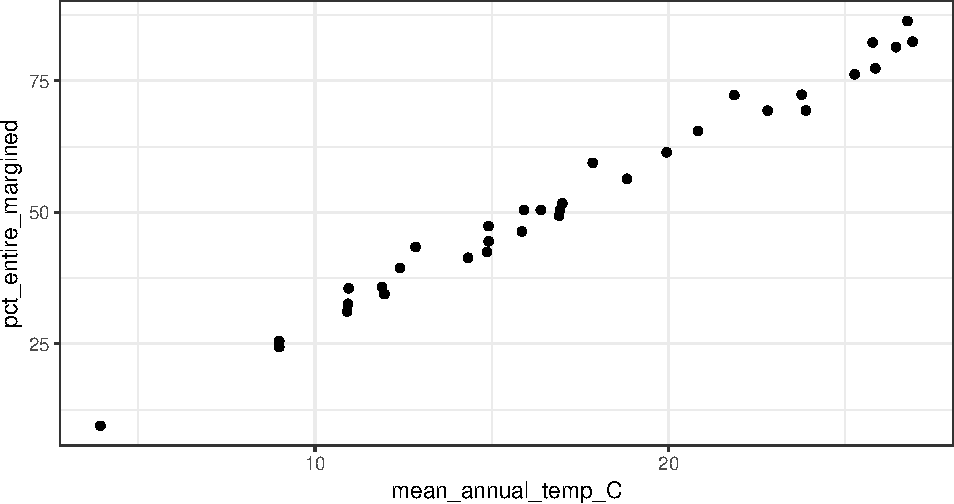
\includegraphics{20190213_mle_slr_files/figure-latex/unnamed-chunk-1-1.pdf}

Let's consider a model for the percent of leaves in the forest canopy as
a function of the mean annual temperature in that forest in degrees
Celsius.

\subsection{Notation and Model
Statement}\label{notation-and-model-statement}

We define the following random variables:

\(Y_i =\) percent of leaves in forest number \(i\) that are entire
margined, \(i = 1, \ldots, n\).

\(X_i =\) mean annual temperature in forest number \(i\) in degrees
Celsius, \(i = 1, \ldots, n\).

We specify our model as follows:

\begin{align*}
(Y_i | X_i = x_i) &= \beta_0 + \beta_1 x_i + \varepsilon_i \\
\varepsilon_i &\simiid \text{Normal}(0, \sigma^2)
\end{align*}

If we condition on the value \(x_i\), then \(\beta_0 + \beta_1 x_i\) is
just a constant. Therefore, we could equivalently state this model as
follows:

\begin{align*}
Y_i | X_i = x_i &\simiid \text{Normal}(\beta_0 + \beta_1 x_i, \sigma^2)
\end{align*}

This is a model for the conditional distribution of the percent of
leaves that are entire margined in a particular forest given the mean
annual temperature in that forest.

The model has three parameters \(\beta_0\), \(\beta_1\), and
\(\sigma^2\). For today, let's pretend that \(\sigma^2\) is a known
constant, and focus on estimation of \(\beta_0\) and \(\beta_1\).

\subsubsection{\texorpdfstring{1. Write down the probability density
function for
\(Y_i | X_i = x_i\).}{1. Write down the probability density function for Y\_i \textbar{} X\_i = x\_i.}}\label{write-down-the-probability-density-function-for-y_i-x_i-x_i.}

\vspace{5cm}

\subsubsection{\texorpdfstring{2. Write down the joint pdf for
\(Y_1, \ldots, Y_n | X_{1} = x_1, \ldots, X_{n} = x_{n}\).}{2. Write down the joint pdf for Y\_1, \textbackslash{}ldots, Y\_n \textbar{} X\_\{1\} = x\_1, \textbackslash{}ldots, X\_\{n\} = x\_\{n\}.}}\label{write-down-the-joint-pdf-for-y_1-ldots-y_n-x_1-x_1-ldots-x_n-x_n.}

\vspace{9cm}

\subsubsection{\texorpdfstring{3. Find the log-likelihood function
\(\ell(\beta_0, \beta_1, \sigma^2 | x_1, y_1, \ldots, x_n, y_n)\)}{3. Find the log-likelihood function \textbackslash{}ell(\textbackslash{}beta\_0, \textbackslash{}beta\_1, \textbackslash{}sigma\^{}2 \textbar{} x\_1, y\_1, \textbackslash{}ldots, x\_n, y\_n)}}\label{find-the-log-likelihood-function-ellbeta_0-beta_1-sigma2-x_1-y_1-ldots-x_n-y_n}

\newpage

\subsubsection{\texorpdfstring{4. Find a critical point of the
log-likelihood function. This will involve taking the partial
derivatives with respect to each of \(\beta_0\) and \(\beta_1\) and
setting the results equal to 0 (remember, we're pretending \(\sigma\) is
a known constant; if we were trying to estimate that too, we would need
to also differentiate with respect to \(\sigma\)). You will have a
system of 2 equations to
solve.}{4. Find a critical point of the log-likelihood function. This will involve taking the partial derivatives with respect to each of \textbackslash{}beta\_0 and \textbackslash{}beta\_1 and setting the results equal to 0 (remember, we're pretending \textbackslash{}sigma is a known constant; if we were trying to estimate that too, we would need to also differentiate with respect to \textbackslash{}sigma). You will have a system of 2 equations to solve.}}\label{find-a-critical-point-of-the-log-likelihood-function.-this-will-involve-taking-the-partial-derivatives-with-respect-to-each-of-beta_0-and-beta_1-and-setting-the-results-equal-to-0-remember-were-pretending-sigma-is-a-known-constant-if-we-were-trying-to-estimate-that-too-we-would-need-to-also-differentiate-with-respect-to-sigma.-you-will-have-a-system-of-2-equations-to-solve.}

You should get answers of the form:

\begin{align*}
\beta_0 &= \frac{1}{n}\sum_{i = 1}^n y_i - \beta_1 \frac{1}{n} \sum_{i = 1}^n x_i = \frac{\left(\sum_{i = 1}^n x_i^2\right) \left(\sum_{i = 1}^n y_i\right) - \left(\sum_{i = 1}^n x_i\right) \left(\sum_{i = 1}^n x_i y_i \right)}{n \sum_{i = 1}^n x_i^2 - \left(\sum_{i = 1}^n x_i\right)^2} \\
\beta_1 &= \frac{n \sum_{i = 1}^n x_i y_i - \left(\sum_{i = 1}^n x_i\right) \left(\sum_{i = 1}^n y_i\right)}{n \sum_{i = 1}^n x_i^2 - \left(\sum_{i = 1}^n x_i\right)^2}
\end{align*}

\vspace{8.25cm}

To formally identify this critical point as a maximum, you'd have to
also verify that the Hessian was negative definite; I won't ask us to do
that in this class.

\subsubsection{\texorpdfstring{5. If you have extra time: In RStudio,
find the maximum likelihood estimates for \(\beta_0\) and \(\beta_1\).
Confirm that your answers match those from the \texttt{lm} function. Add
a plot of the estimated regression line to the scatterplot (consider
using
\texttt{geom\_abline}).}{5. If you have extra time: In RStudio, find the maximum likelihood estimates for \textbackslash{}beta\_0 and \textbackslash{}beta\_1. Confirm that your answers match those from the lm function. Add a plot of the estimated regression line to the scatterplot (consider using geom\_abline).}}\label{if-you-have-extra-time-in-rstudio-find-the-maximum-likelihood-estimates-for-beta_0-and-beta_1.-confirm-that-your-answers-match-those-from-the-lm-function.-add-a-plot-of-the-estimated-regression-line-to-the-scatterplot-consider-using-geom_abline.}

\subsubsection{\texorpdfstring{6. If you have even more extra time:
Argue that maximizing the log-likelihood function from part 3 is
equivalent to minimizing the sum of squared errors
\(SSE = \sum_{i = 1}^n \left\{y_i - (\beta_0 + \beta_2 x_{i}) \right\}^2\).
Thus, for this model, maximum likelihood is equivalent to estimating the
coefficients by ordinary least
squares.}{6. If you have even more extra time: Argue that maximizing the log-likelihood function from part 3 is equivalent to minimizing the sum of squared errors SSE = \textbackslash{}sum\_\{i = 1\}\^{}n \textbackslash{}left\textbackslash{}\{y\_i - (\textbackslash{}beta\_0 + \textbackslash{}beta\_2 x\_\{i\}) \textbackslash{}right\textbackslash{}\}\^{}2. Thus, for this model, maximum likelihood is equivalent to estimating the coefficients by ordinary least squares.}}\label{if-you-have-even-more-extra-time-argue-that-maximizing-the-log-likelihood-function-from-part-3-is-equivalent-to-minimizing-the-sum-of-squared-errors-sse-sum_i-1n-lefty_i---beta_0-beta_2-x_i-right2.-thus-for-this-model-maximum-likelihood-is-equivalent-to-estimating-the-coefficients-by-ordinary-least-squares.}


\end{document}
